\section{Results}

\end{multicols}
	
\begin{table}[H]
\centering
\label{tab:results-summary}
\begin{tabular}{llcc}
\toprule
Model & Technique & Macro F1 & Balanced Acc. \\
\midrule
\multicolumn{4}{l}{\textbf{Traditional ML}} \\
Decision Tree & -- & 0.675 & 0.685 \\
Random Forest & -- & 0.720 & 0.719 \\
Gradient Boosting & -- & 0.722 & 0.718 \\
Support Vector Machine & -- & 0.652 & 0.635 \\
K-Nearest Neighbors & -- & 0.601 & 0.595 \\
MLP Classifier & -- & 0.678 & 0.676 \\
ELM Classifier & -- & 0.645 & 0.630 \\
\addlinespace
\multicolumn{4}{l}{\textbf{LLMs}} \\
Qwen2.5-3B & 0-shot & 0.218 & 0.297 \\
Qwen2.5-3B & 1-shot & 0.387 & 0.562 \\
Qwen2.5-3B & 5-shot & 0.306 & 0.377 \\
Meta-Llama3-9B & 0-shot & 0.280 & 0.341 \\
Meta-Llama3-9B & 1-shot & 0.392 & 0.509 \\
Meta-Llama3-9B & 5-shot & 0.481 & 0.494 \\
\bottomrule
\end{tabular}
\caption{Summary of traditional ML and LLM performance on the test set (Macro F1 and Balanced Accuracy).}
\end{table}
	
\begin{figure}[H]
\centering
	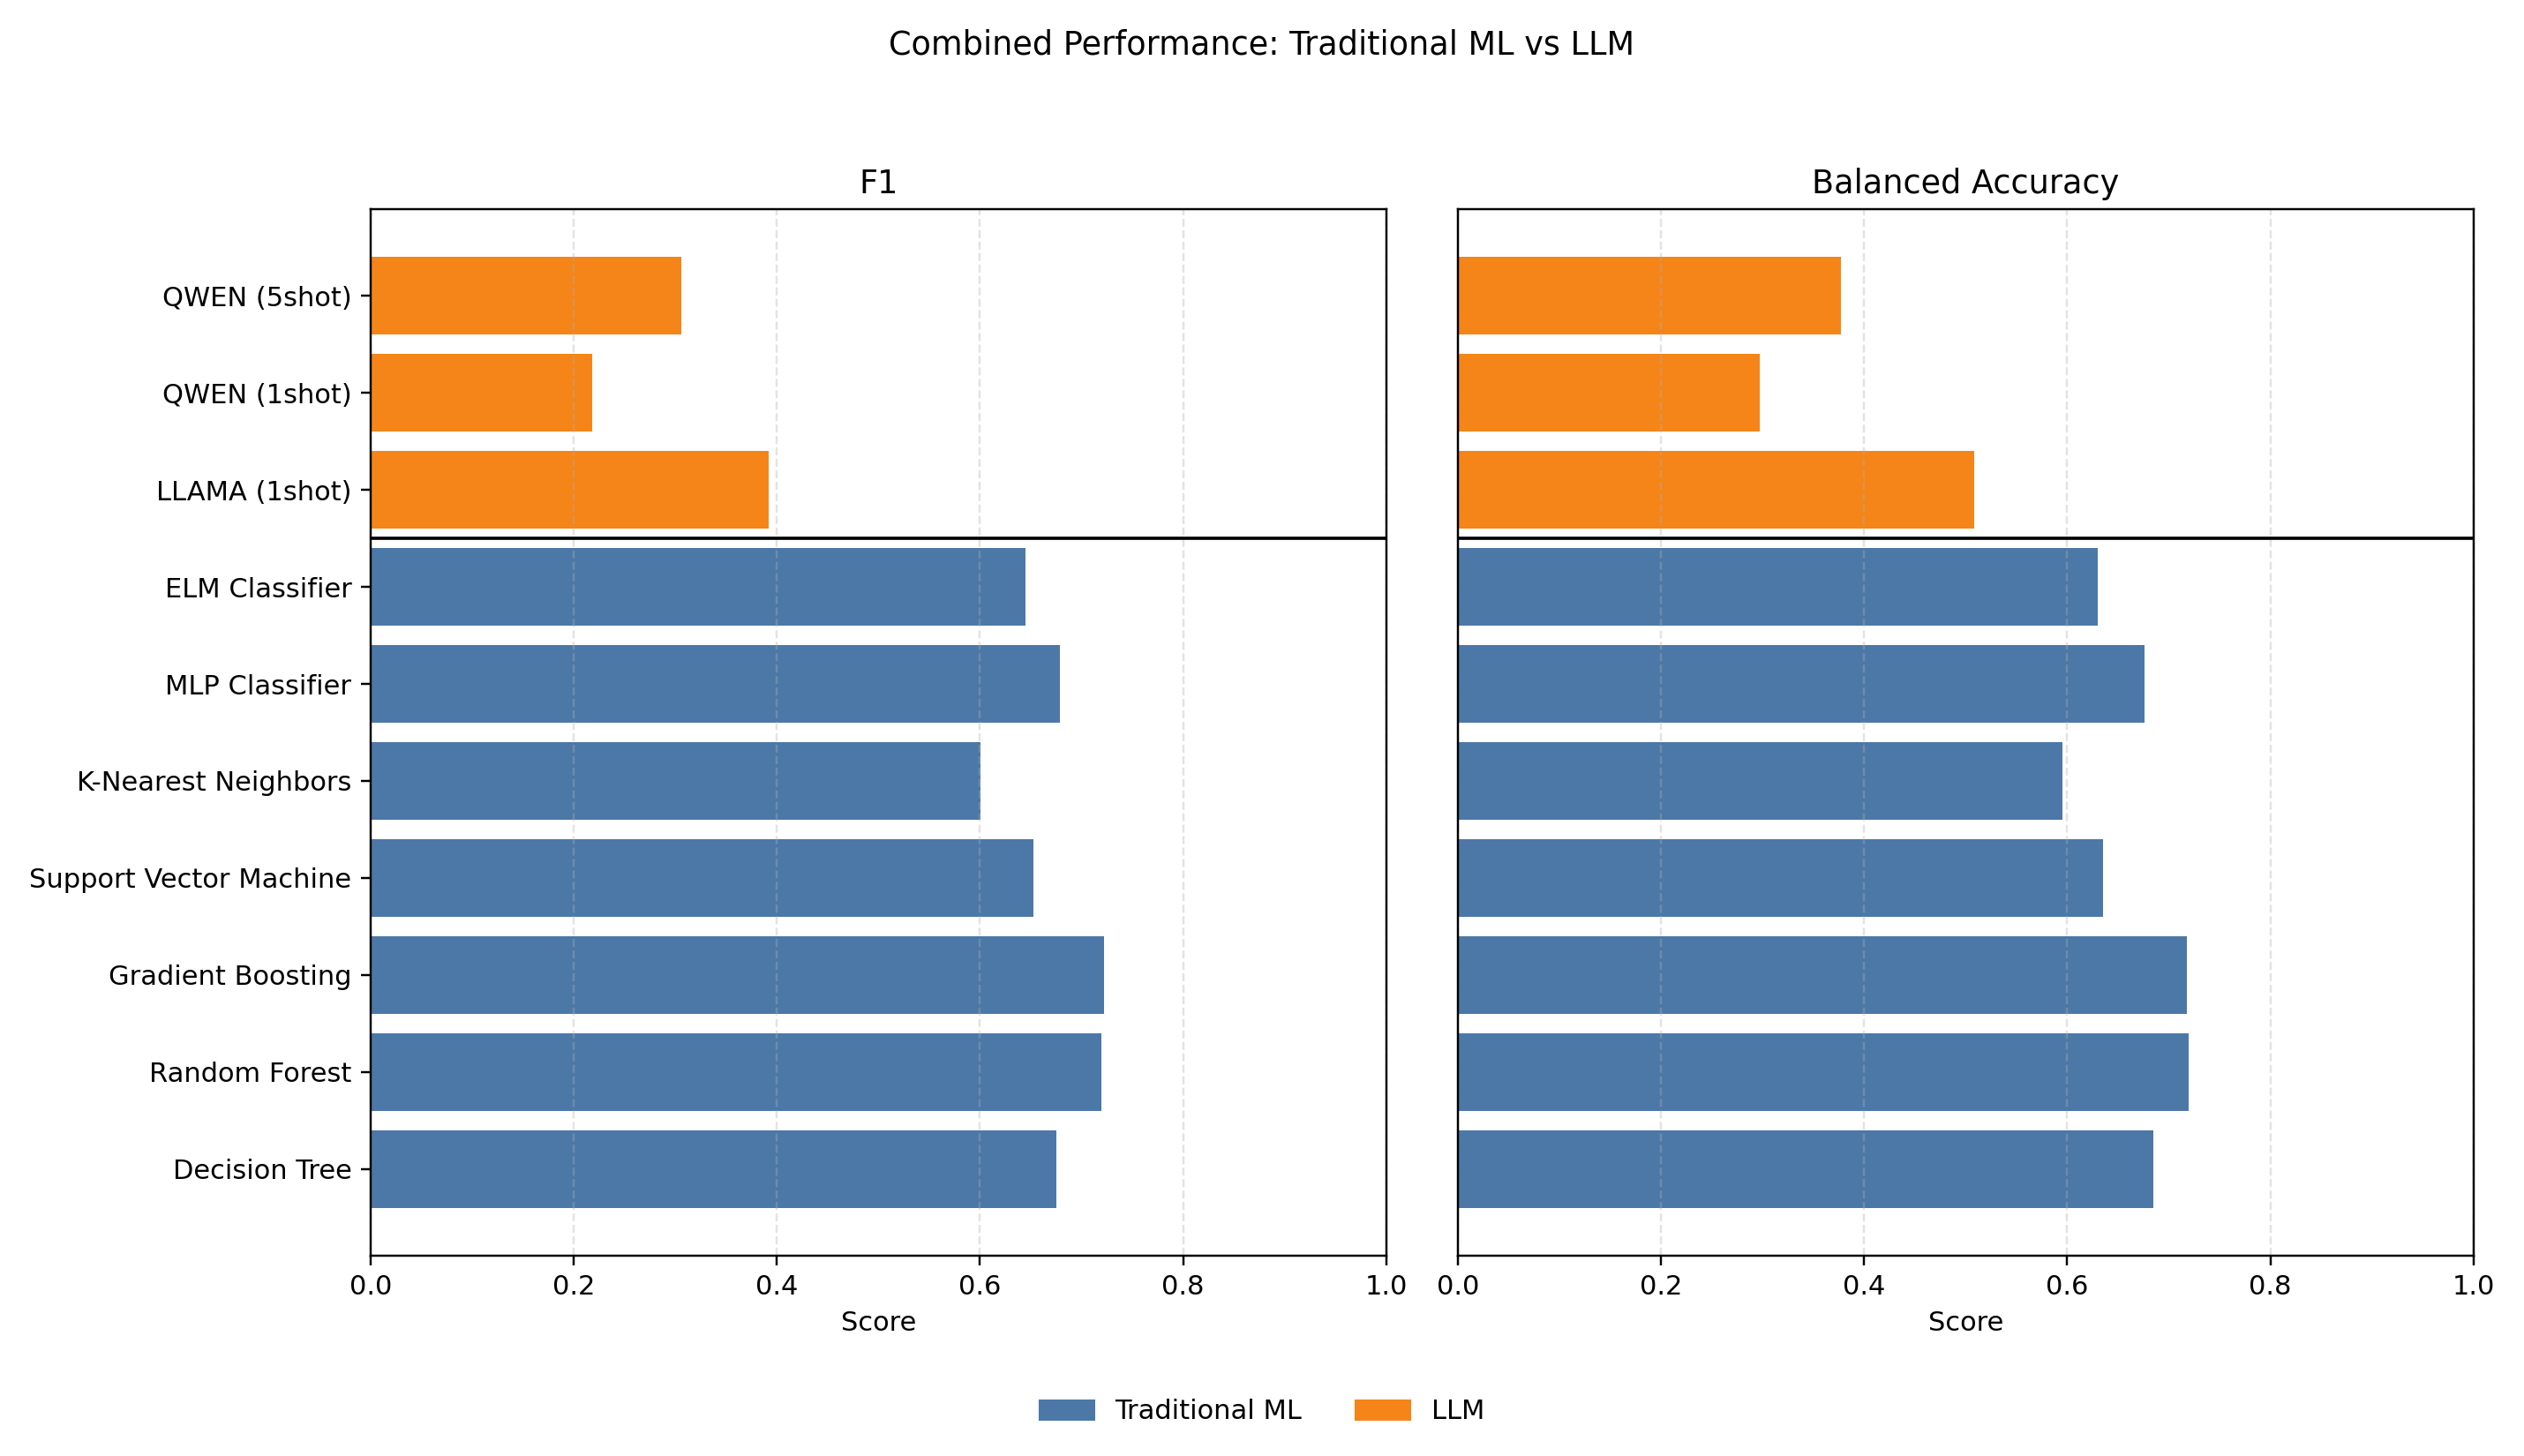
\includegraphics[width=\textwidth]{code/plots/combined_tradml_llm_performance.png}
	\caption{Combined performance comparison of traditional machine learning models and large language models using F1 and Balanced Accuracy.}
\end{figure}

\begin{figure}[H]
\centering
	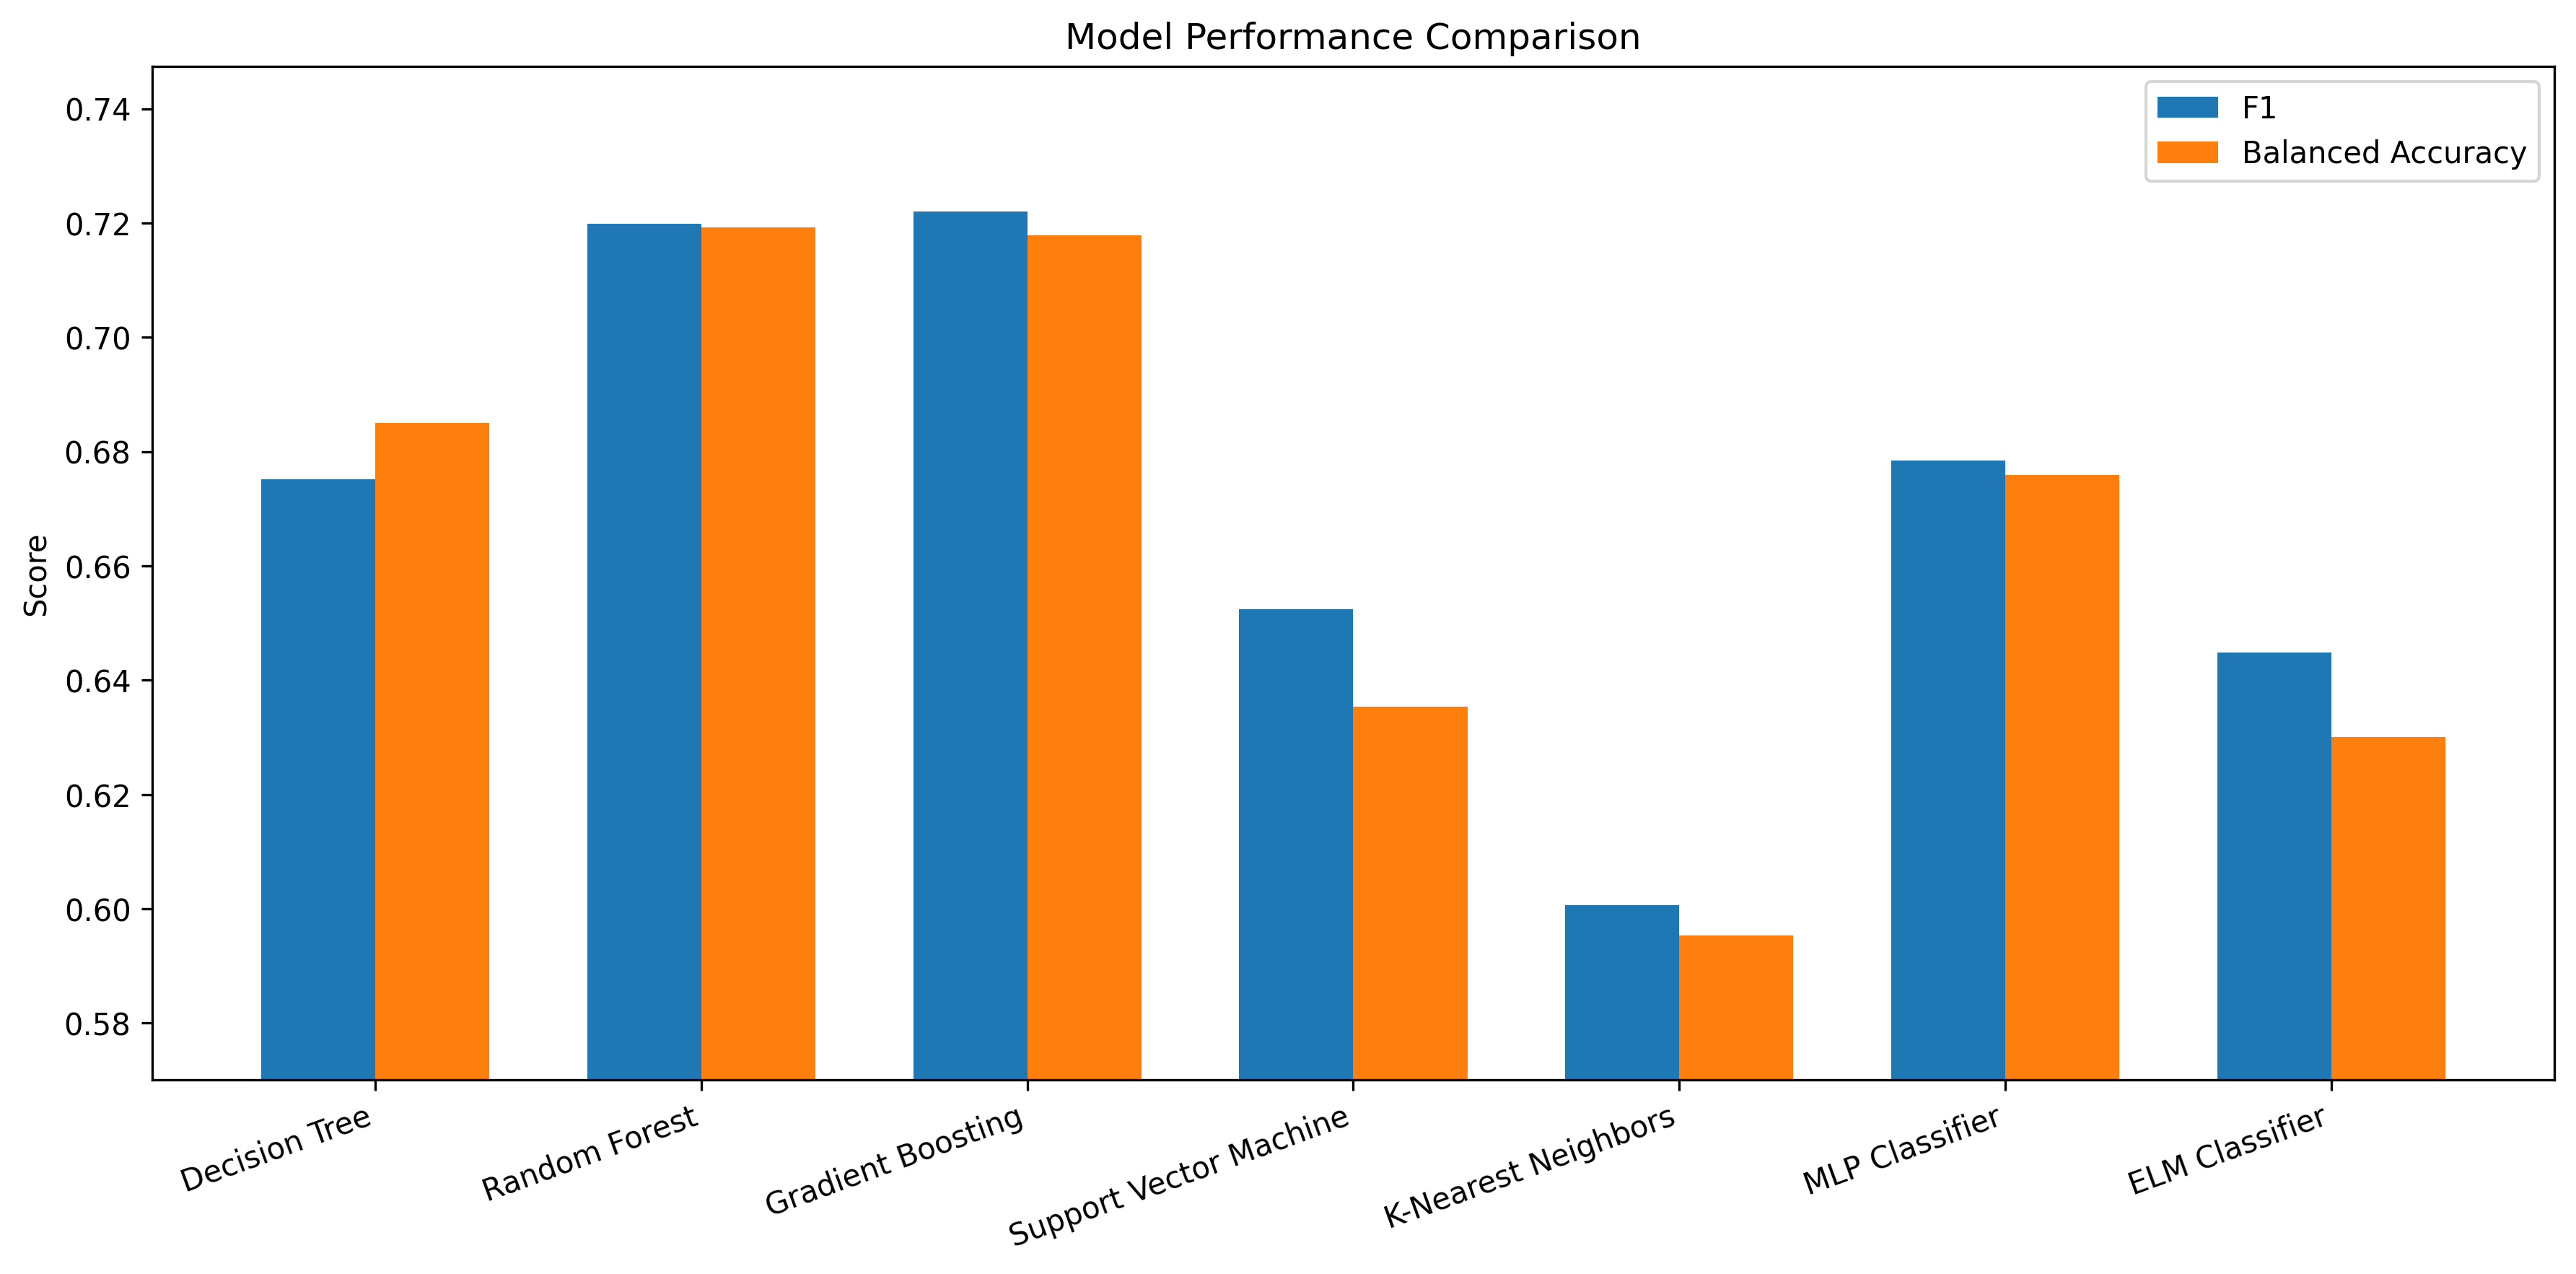
\includegraphics[width=\textwidth]{code/plots/model_performance_py.png}
	\caption{Test-set performance comparison of traditional predictive models using Macro F1 and Balanced Accuracy.}
\end{figure}

\begin{multicols}{2}

\subsection{Traditional Predictive Models}
Various traditional model architectures are implemented. The evaluated models are Random Forest, Decision Tree, Support Vector Machine, Gradient Boosting, K-Nearest Neighbors, Extreme Learning Machine, and Multi-layer Perceptron. The performance of each model is measured using plain accuracy, balanced accuracy, and F1 score. The accuracy of a model can be calculated as
\[
	\frac{\text{True Positive} + \text{True Negative}}{\text{Total Prediction}}.
\]
It is an intuitive measure of how correct the model predictions are, but falls short when the given dataset is imbalanced. To mitigate this issue, the balanced accuracy is preferred:
\[
	\frac{\text{Sensitivity} + \text{Specificity}}{2}.
\]
In addition, the F1 score is also utilized, calculated as the harmonic mean of precision and recall:
\[
	\frac{2 \times \text{Precision} \times \text{Recall}}{\text{Precision} + \text{Recall}}.
\]
As shown in Fig. 1, the model performance plot summarizes the comparative results across all evaluated traditional predictive models. We can see that ensemble methods remain the top performers, with Gradient Boosting and Random Forest achieving the highest F1 scores of 0.722 and 0.720, respectively. Support Vector Machine and Extreme Learning Machine also show competitive performance, while K-Nearest Neighbors has the lowest F1 score among the traditional models at 0.601. These results are consistent with existing literature that highlights the effectiveness of ensemble methods in classification tasks, particularly in educational contexts where complex interactions between features are common.

\subsection{Large Language Models}
\begin{figure}[H]
	\centering
	\begin{minipage}{0.5\textwidth}
		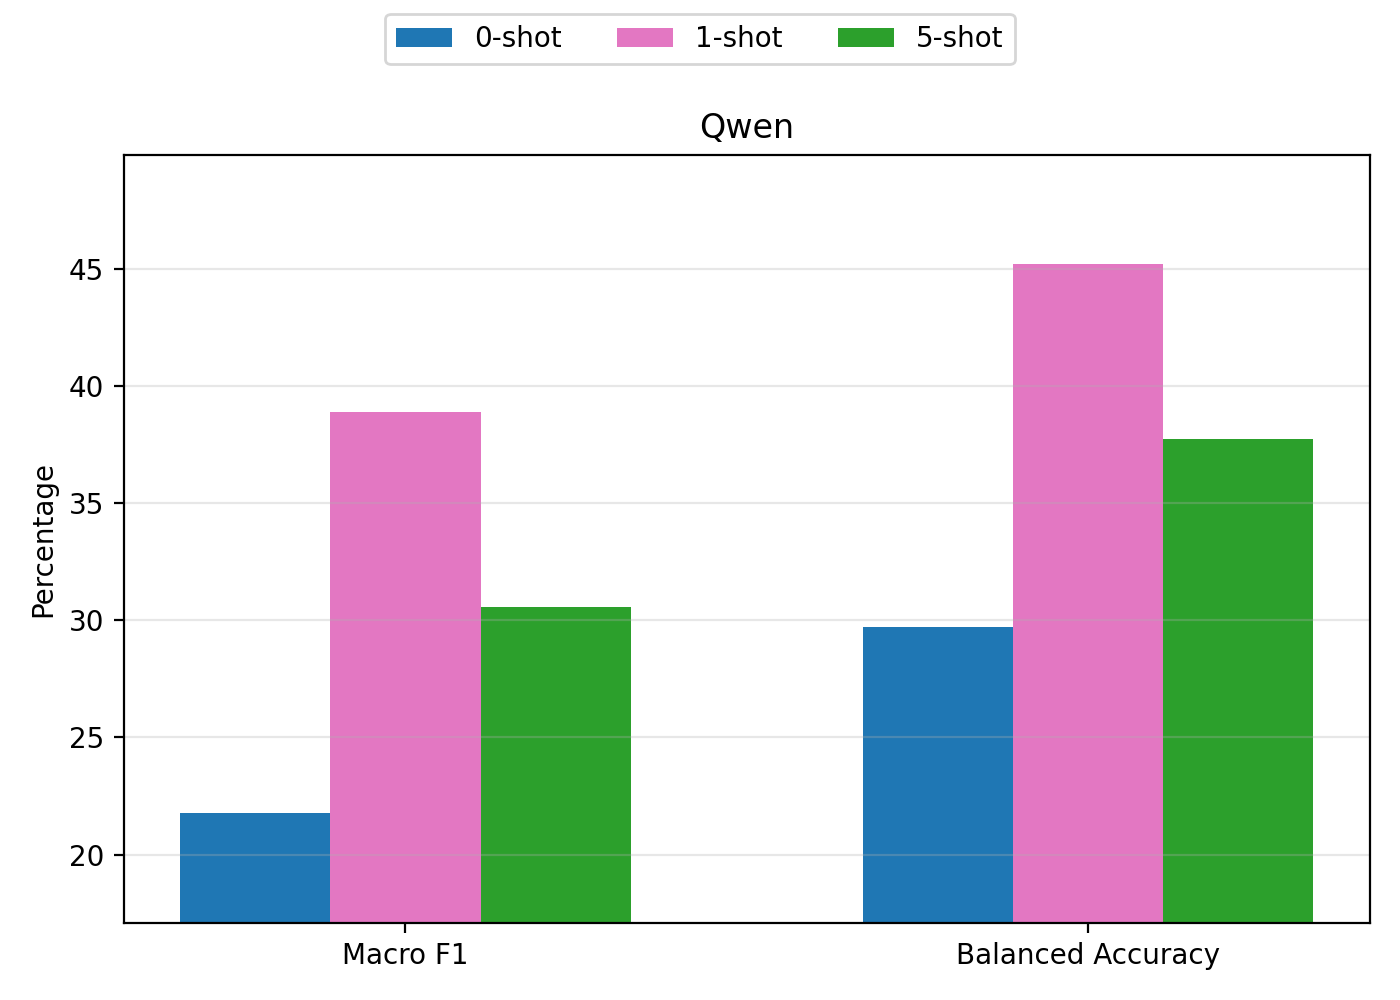
\includegraphics[width=\textwidth]{code/plots/qwen_metric_technique_comparison.png}
	\end{minipage}
	\begin{minipage}{0.5\textwidth}
		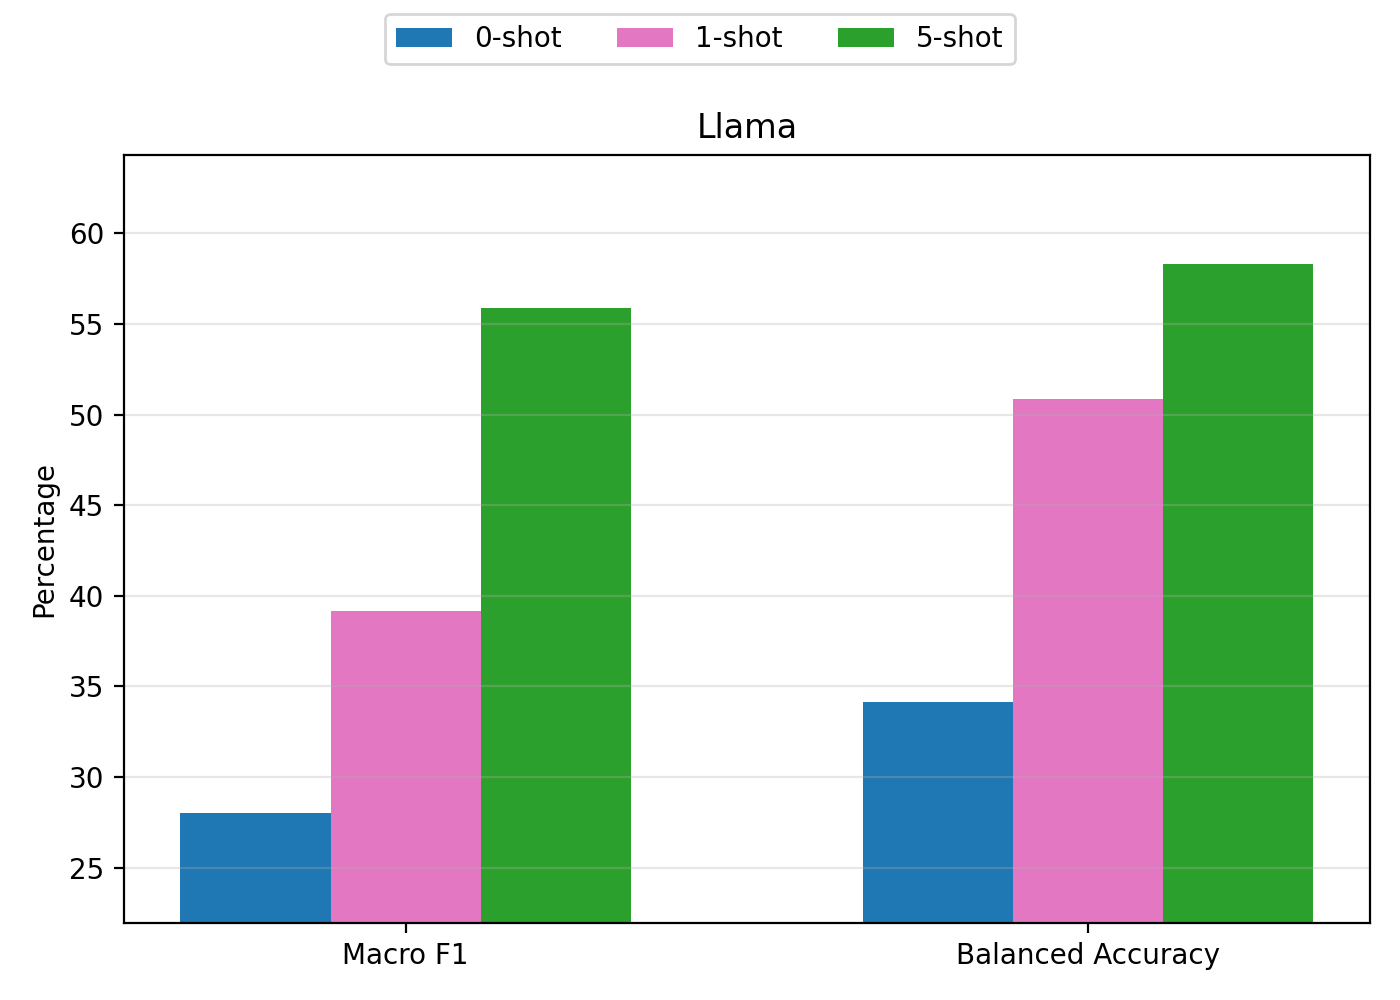
\includegraphics[width=\textwidth]{code/plots/llama_metric_technique_comparison.png}
	\end{minipage}
	\caption{Prompting-technique comparison for Qwen2.5-3B (left) and Meta-Llama3-9B (right), using Macro F1 and Balanced Accuracy.}
\end{figure}
We use a modified metric for LLMs---Macro F1. This metric effectively treats each class in a model equally important by taking the mean of the F1 scores of each class. This is particularly useful in our case, where the dataset is imbalanced, and we want to ensure that the model's performance on the minority class (e.g., at-risk students) is not overshadowed by its performance on the majority class (e.g., passing students). As shown in Fig. 1, the best performing LLM configuration is Qwen-2.5-3B with 5-shot prompting, which achieves a Macro F1 score of 0.45 and a balanced accuracy of 0.377, a performance no better than random guessing. The other LLM configurations perform even worse, with Macro F1 scores ranging from 0.218 to 0.392 and balanced accuracies between 0.297 and 0.562. 

Even the best performing LLM configuration (Qwen-2.5-3B with 5-shot prompting) achieves a Macro F1 score of only 0.45, which is significantly lower than the lowest scoring traditional model (KNN with an F1 score of 0.85). This suggests that the bottleneck is not model capacity — LLaMA-3-8B has 8 billion parameters compared to KNN's zero learned parameters — but rather the fundamental mismatch between LLM pretraining distribution (natural language) and the input modality (serialized numerical feature vectors).

This gap also contextualizes the practical implications for HEIs: at current scales, deploying general-purpose LLMs for student outcome classification without fine-tuning would produce predictions no better than a majority-class baseline, rendering them unsuitable for early-warning systems where per-class sensitivity is critical.